\documentclass{beamer}
% \usepackage{animate}
\usepackage{multimedia}
\usepackage[english,russian]{babel}

\usepackage{pgfpages}
\setbeameroption{show notes on second screen}
%https://tug.ctan.org/macros/latex/contrib/beamer/doc/beameruserguide.pdf

\usepackage[T2A]{fontenc}
\usepackage[utf8]{inputenc}

\setbeamertemplate{caption}[numbered]

\usetheme{CambridgeUS}
\usecolortheme{dolphin}


\title[Введение в КГ]{Введение в компьютерную графику}
\author[Быковских Д.А.]{Быковских Дмитрий Александрович}
\date{05.09.2026}

\begin{document}
	\begin{frame}
		\titlepage
	\end{frame}
	%\section{Обзор}
	\begin{frame}{Содержание}
		\begin{itemize}
			\item 
			Общее представление о компьютерной графике
			\item
			Способы представления графических данных
			\item
			Некоторые факты из истории компьютерной графики
		\end{itemize}

		\note{
			\begin{figure}
				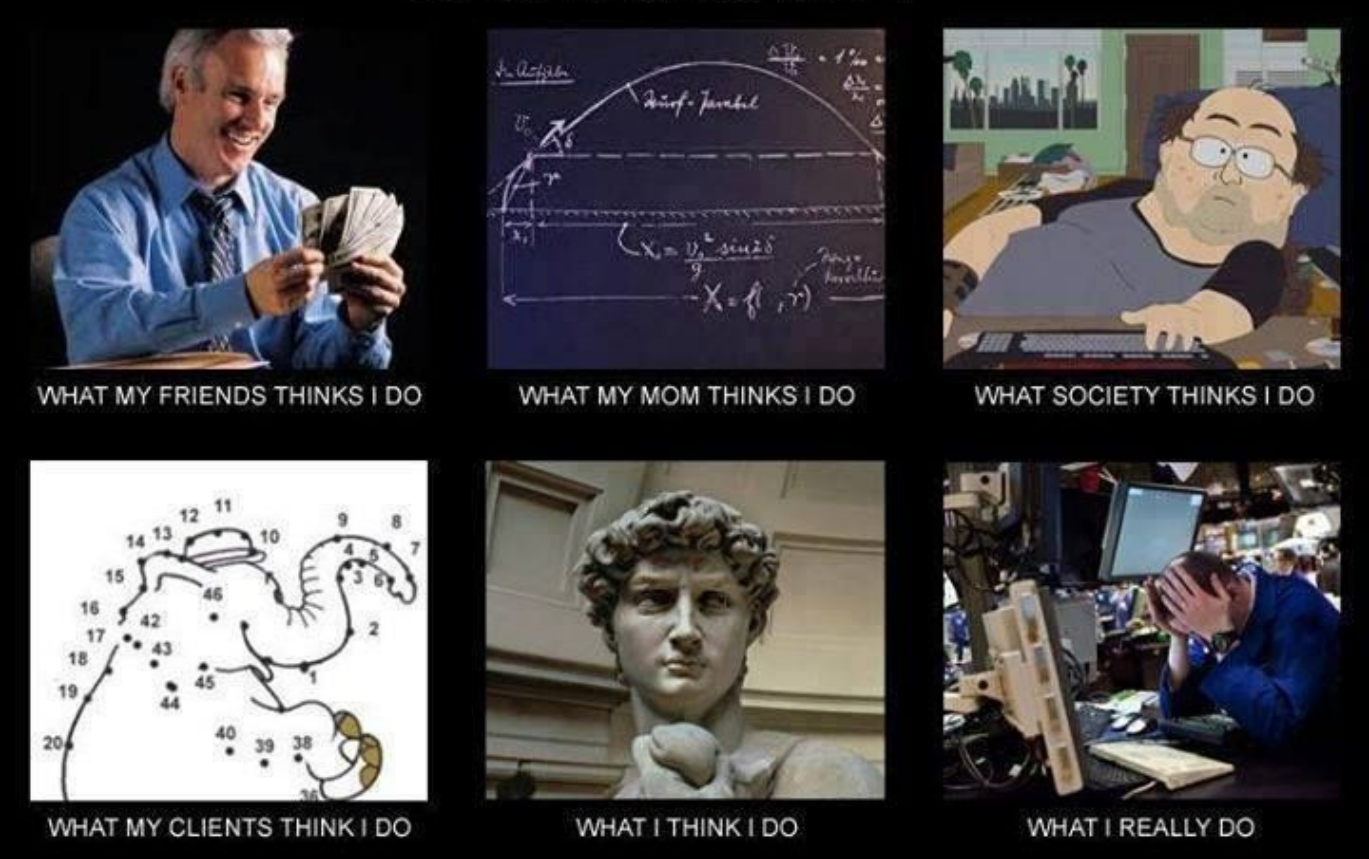
\includegraphics[width=0.8\textwidth]{images/cg_work_meme.png}
				\caption{Изображение для привлечения внимания}
			\end{figure}
		}
	\end{frame}
	\begin{frame}{Что такое компьютерная графика (КГ)?}
		\textbf{Компьютерная графика} --- междисциплинарная область информатики, изучающая математические и вычислительные основы генерации, обработки, представления и визуализации изображений и геометрической информации с использованием вычислительных систем.

		% Компьютерная графика --- одно из направлений информационных технологий, которое занимается созданием, редактированием и визуализацией \textbf{графических изображений}.
		{
			\small
			Спектр применений:
			\vskip-4mm
			\begin{columns}[t]
				\begin{column}{0.48\textwidth}
					{\footnotesize
						\begin{itemize}
							\item Разработка компьютерных игр (виртуальный мир, персонажи, эффекты)
							\item Визуализация данных (диаграммы, графики)
							\item Дизайн (логотипы, баннеры, упаковка, интерфейсы)
							\item Симуляция и моделирование (виртуальные среды для тестирования)
						\end{itemize}
					}
				\end{column}
				\begin{column}{0.48\textwidth}
					{\footnotesize
						\begin{itemize}
							\item Анимация (фильмы, видеоролики, реклама)
							\item Медицинская визуализация (модели органов, тканей)
							\item Архитектурное проектирование (модели зданий, интерьеров)
							\item Редактирование фото- и видеоматериалов (улучшение качества)
							\item и многое другое
						\end{itemize}
					}
				\end{column}
			\end{columns}
		}
		\note{

		\textbf{Машинная графика (Computer graphics, ГОСТ 27459-87)} --- совокупность методов и приемов для преобразования при помощи ЭВМ данных в графическое представление или графического представления в данные.

		}
		
		\if 0
		3D-моделирование и анимация: Создание трехмерных моделей объектов, персонажей и сцен, а также их анимация для использования в фильмах, играх, визуализации архитектурных проектов и многих других областях.
		
		2D-графика и иллюстрации: Создание двумерных изображений, иллюстраций, рисунков, артов и графических элементов для книг, журналов, рекламы и дизайна.
		
		Визуализация данных: Преобразование сложных данных в наглядные и понятные визуальные формы, такие как графики, диаграммы, инфографика и карты.
		
		Компьютерная анимация и эффекты: Создание анимаций, спецэффектов и визуальных элементов для фильмов, рекламы, игр и других медийных продуктов.
		
		Графический дизайн: Разработка дизайна логотипов, брендинга, упаковки, веб-сайтов, приложений и других визуальных элементов.
		
		Виртуальная реальность (VR) и дополненная реальность (AR): Создание виртуальных и дополненных миров, в которых пользователи могут взаимодействовать и иметь визуальный опыт.
		
		Компьютерное моделирование: Создание компьютерных моделей и симуляций для изучения поведения систем, процессов и явлений в науке, инженерии и других областях.
		
		Медицинская визуализация: Создание графических изображений и моделей для обучения, диагностики и планирования медицинских процедур.
		
		Архитектурная визуализация: Создание виртуальных моделей зданий и помещений для архитекторов и дизайнеров.
		
		Ретушь и обработка фотографий: Использование графических инструментов для улучшения и изменения фотографий.
		
		Генеративное искусство: Использование алгоритмов и программирования для создания уникальных искусственных изображений и анимаций.
		\fi
		
	\end{frame}


	\begin{frame}{Основные направления}
		
		\begin{columns}
			\begin{column}{0.3\textwidth}
				
				\textbf{Image Processing}
				
				Image Compression
				
				Noise Reduction

				\begin{figure}
				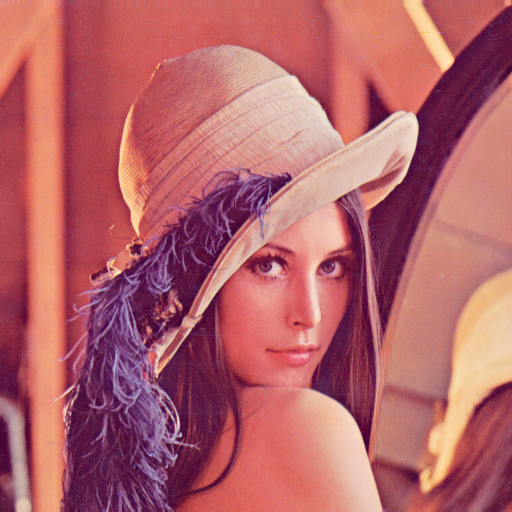
\includegraphics[width=\textwidth]{images/Lenna_test_image.png}
				\caption{Эталонное изображение (Söderberg Lenna)}
				\end{figure}
				
			\end{column}

			\begin{column}{0.4\textwidth}
				
				\textbf{Rendering}
				
				Rasterization / Ray tracing

				Non-photorealistic rendering

				\begin{figure}
				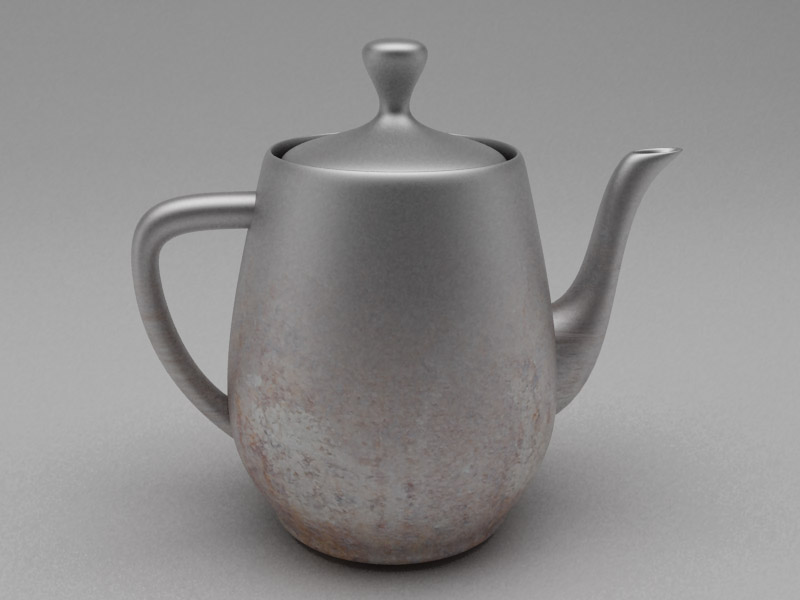
\includegraphics[width=\textwidth]{images/Utah_teapot.png}
				\caption{Классическая модель рендеринга (чайник Ньюэлла, чайник из Юты)}
				\end{figure}
				
			\end{column}

			\begin{column}{0.3\textwidth}
				
				\textbf{Computer Vision}
				
				Vision for robotics

				Object recognition

				Appearance representations

				\vspace{2.5mm}

				\begin{figure}
				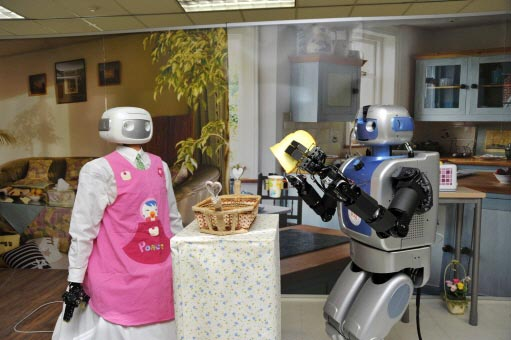
\includegraphics[width=\textwidth]{images/Computer_vision.png}
				\caption{Компьютерное зрение в робототехнике (семейная пара)}
				\end{figure}
			\end{column}
			
		\end{columns}

		\note{
			

			% Самые популярные направления на сегодняшний день: 
			% \begin{itemize}
			% 	\item рендеринг;
			% 	\item анимация и симуляция;
			% 	\item геометрическое моделирование;
			% 	\item машинное обучение и ИИ;
			% 	\item виртуальная и дополненная реальность;
			% 	\item научная визуализация;
			% 	\item вычислительная фотография. 
			% \end{itemize}



			Другие популярные направления из Computer Graphics (ACM Digital Library and Computing Classification System)
			\vspace{0.5em}

			\begin{columns}
				\scriptsize
				\begin{column}{0.4\textwidth}
					Graphics systems and interfaces
					\begin{itemize}
						\itemsep0pt
						\parsep0pt
						\topsep1pt
						\partopsep0pt
						\item Graphics processors
						\item Virtual / mixed / augmented reality
						\item Graphics devices
						\item Graphics file formats
					\end{itemize}
					Image manipulation
					\begin{itemize}
						\itemsep0pt
						\parsep0pt
						\topsep1pt
						\partopsep0pt
						\item Computational photography
						\item Image processing
						\item Antialiasing
						\item Texturing
						\item Image-based rendering
					\end{itemize}
				\end{column}
				\begin{column}{0.4\textwidth}
					Shape modeling
					\begin{itemize}
						\itemsep0pt
						\parsep0pt
						\topsep1pt
						\partopsep0pt
						\item Mesh models
						\item Mesh geometry models
						\item Parametric curve and surface models
						\item Point-based models
						\item Volumetric models
						\item Shape analysis
					\end{itemize}
					Animation
					\begin{itemize}
						\itemsep0pt
						\parsep0pt
						\topsep1pt
						\partopsep0pt
						\item Procedural animation
						\item Physical simulation
						\item Motion capture/processing
					\end{itemize}

				\end{column}
			\end{columns}
		}

		\end{frame}

	\section{Способы представления графических данных}

	\begin{frame}{Растровая графика}
		\begin{figure}
			\href{https://creativeyatra.com/news/windows-ends-journey-ms-paint-three-decades}{
				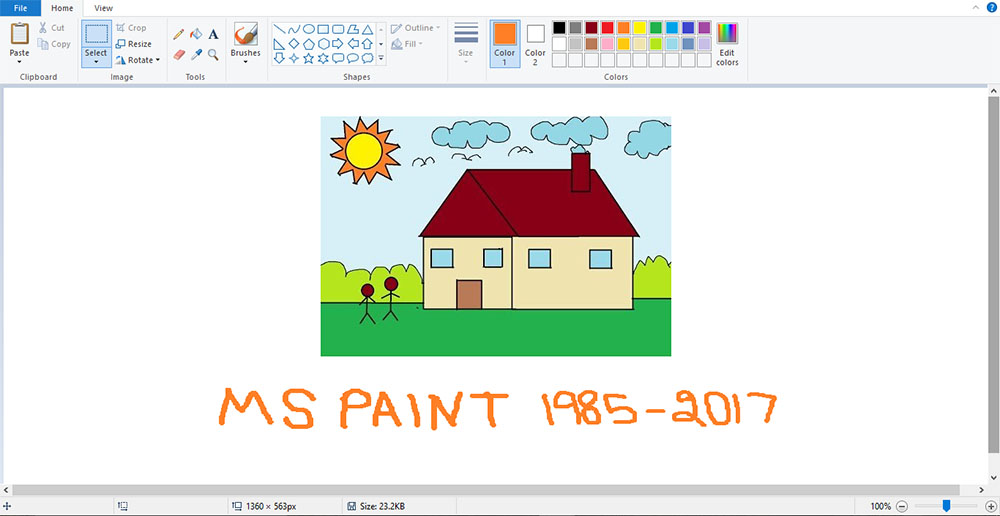
\includegraphics[width=0.98\textwidth]{images/MS_Paint.jpg}}
			\caption{MS Paint}
		\end{figure}
	
		\note{
			\textbf{Растровая графика (bitmap или pixel-based)} представляет изображение в виде массива пикселей.
			Каждый пиксель хранит информацию о цвете; расположенные в определённом порядке, пиксели формируют изображение.
	
			Качество изображения зависит от количества пикселей.
			Чем выше разрешение (количество пикселей на единицу площади), тем детализированнее изображение.
		}
	\end{frame}
	
	\begin{frame}{Векторная графика}
		\begin{figure}
			\href{https://www.gimp.org/}{
				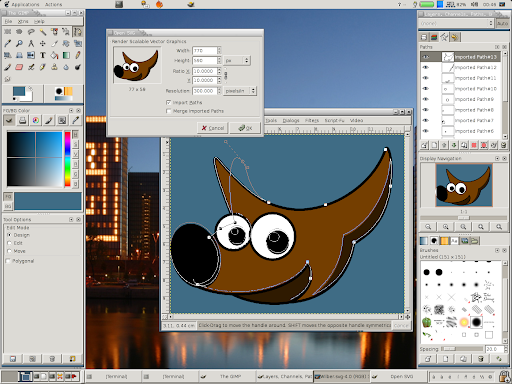
\includegraphics[width=0.7\textwidth]{images/GIMP.png}}
			\caption{GIMP (GNU Image Manipulation Program)}
		\end{figure}
	
		\note{
			\textbf{Векторная графика} представляет изображение, состоящее из примитивов и/или математических объектов (линий, точек, треугольников, кривых, поверхностей и др.).
			Эти объекты описываются с помощью набора параметров и/или уравнений, что позволяет масштабировать изображение без потери качества.
			
			GIMP на слайде --- растровый редактор, но работает с векторными элементами.
		}
	\end{frame}
	
	\begin{frame}{Воксельная графика}
		\begin{figure}
			\href{https://ephtracy.github.io}{
				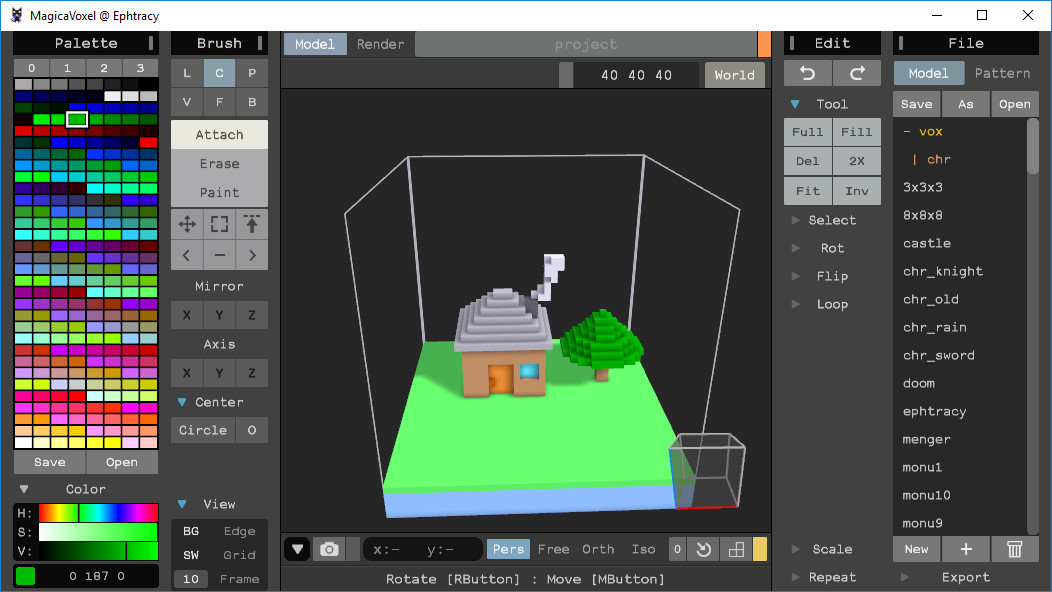
\includegraphics[width=0.9\textwidth]{images/MagicaVoxel.jpg}}
			\caption{MagicaVoxel --- редактор воксельной графики}
		\end{figure}
	
		\note{
			\textbf{Воксельная графика} --- трёхмерный аналог растровой графики, где изображение состоит из объёмных пикселей, называемых вокселями (англ.\ voxel --- volume element).
			Воксели представляют собой кубические блоки, которые формируют объёмные объекты в 3D-пространстве.
		}
	\end{frame}
	
	\begin{frame}{Gaussian Splatting (2023)}
		\begin{figure}
			\href{https://www.youtube.com/watch?v=ERuRMOVO58Q}{
				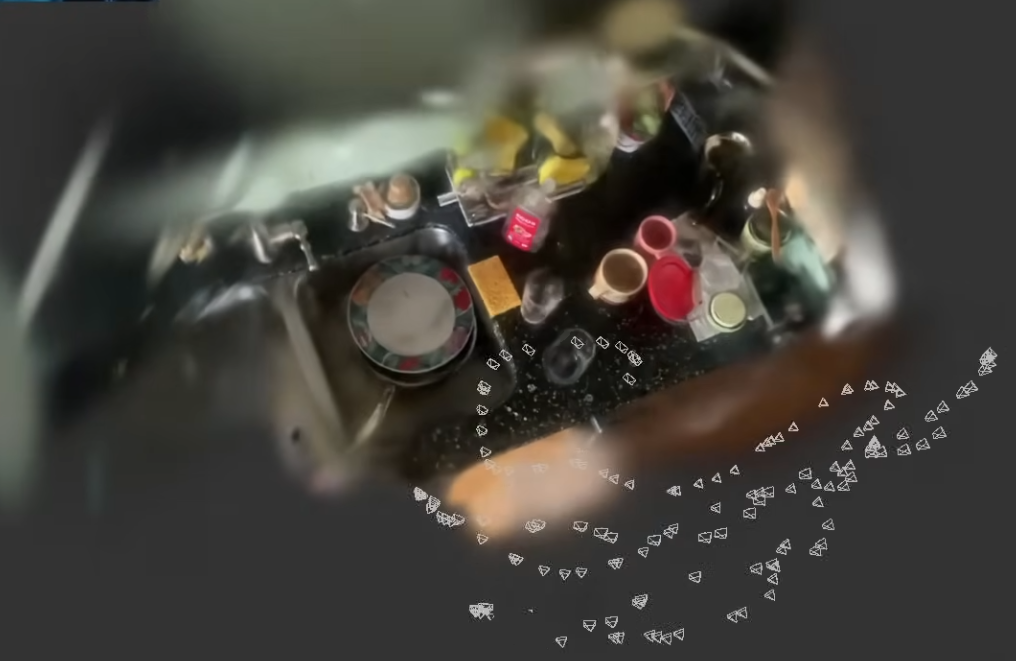
\includegraphics[width=0.8\textwidth]{images/3DGS.png}}
			\caption{Процесс построения изображения с помощью Gaussian Splatting}
		\end{figure}
	
		\note{
			{\footnotesize
			\textbf{3D Gaussian (3D-гауссиан)} --- трёхмерный объект (<<эллипсоид>>), который описывается следующей формулой:
			
			\[
				G(x, \mu, \Sigma) = \frac{1}{\sqrt{(2\pi)^3 \det(\Sigma)}} \exp\left(-\frac{1}{2} (x - \mu)^T \Sigma^{-1} (x - \mu)\right),
			\]
				
			где $\mu$ --- центр; 
			$\Sigma = RSS^TR^T$ --- ковариационная матрица (форма и ориентация);
			$R$ --- поворот;
			$S$ --- масштаб.
		
			
			\textbf{Splatting (сплаттинг)} --- техника рендеринга, при которой 3D-примитивы проецируются на 2D-экран как <<кляксы>> с размытием.
		
			\textbf{Наложение полупрозрачных гауссианов (alpha blending)} рассчитывается как:
			\[
				c(r) = \sum_{i \in N} c_i \sigma_i \prod_{j=1}^{i-1} (1 - \sigma_j),
			\]
			где $r$ --- луч взгляда;
			$c_i$ --- цвет $i$-го гауссиана, рассчитываемый с помощью сферических гармоник;
			$\sigma_i = \alpha_i \cdot G_i$; $\alpha_i$ --- непрозрачность $i$-го гауссиана;
			$N$~---~упорядоченное по глубине множество гауссианов вдоль луча.
			}
		}
	\end{frame}

	
	\section{История развития. Интересные факты}

\if 0	
	\begin{frame}
	%https://iasl.uni-muenchen.de/links/GCA-IV.2e.html
	%https://www.timetoast.com/timelines/6248910a-e70f-4a32-b27c-e13ef9c355dc
	%https://web.archive.org/web/20070405181508/http://accad.osu.edu/\%7Ewaynec/history/lesson2.html
	%https://web.archive.org/web/20051103164835/http://accad.osu.edu/~waynec/history/lesson2.html
	

	История компьютерной графики насчитывает несколько десятилетий и прошла через ряд важных этапов и достижений. Вот краткий обзор этой истории:
	
	1950-е годы: Ранние исследования в области компьютерной графики начались в 1950-х годах. В 1950 году Иван Сазерленд (Ivan Sutherland) создал устройство "Скетчпад" (Sketchpad), позволяющее рисовать графику с помощью светового пера и дисплея.
	
	1960-е годы: В 1963 году Сазерленд представил прототип первого компьютерного графического устройства для рисования 3D-изображений, названного "TX-2 Sketchpad". Этот момент считается началом трехмерной компьютерной графики.
	
	1970-е годы: В 1970-х годах были разработаны первые программы для создания и редактирования графики, такие как "SuperPaint" и "Computer Graphics System" на основе аппаратных решений. Были также созданы первые алгоритмы заполнения и отсечения для растровой графики.
	
	1980-е годы: В это десятилетие произошли значительные прорывы в компьютерной графике. Были разработаны первые графические интерфейсы пользователя (GUI), например, интерфейс для компьютера Apple Macintosh. Также были созданы первые 3D-моделирование и анимационные программы.
	
	1990-е годы: С распространением персональных компьютеров и улучшением аппаратного обеспечения появились новые возможности для компьютерной графики. Были разработаны 3D-игры, программы для редактирования фотографий и видеороликов.
	
	2000-е годы: Развитие 3D-графики продолжилось, и стали доступны более мощные инструменты для создания сложных 3D-моделей и анимаций. Также стали популярными виртуальная и дополненная реальность.
	
	2010-е годы: Продолжалось усовершенствование компьютерной графики, включая разработку более реалистичных графических движков для видеоигр, прорывы в области визуализации данных и рост популярности анимации и цифрового искусства.
	
	\end{frame}
\fi
	
	
	\begin{frame}{Spacewar (1962 г.)}{Одна из первых компьютерных игр}
	
	\begin{columns}
		
		\begin{column}{0.5\textwidth}
			
			%Название: Spacewar!
			
			\textbf{Жанр:} Shoot’em up, космический симулятор
			
			\textbf{Авторы:} Steve Russell, Martin Graetz, Wayne Wiitanen, Bob Saunders, Steve Piner
			
			\textbf{Платформа:} DEC PDP-1
			
			\textbf{Время разработки:} $\approx$200 ч
			
		\end{column}
		\begin{column}{0.5\textwidth}
			\begin{figure} 
			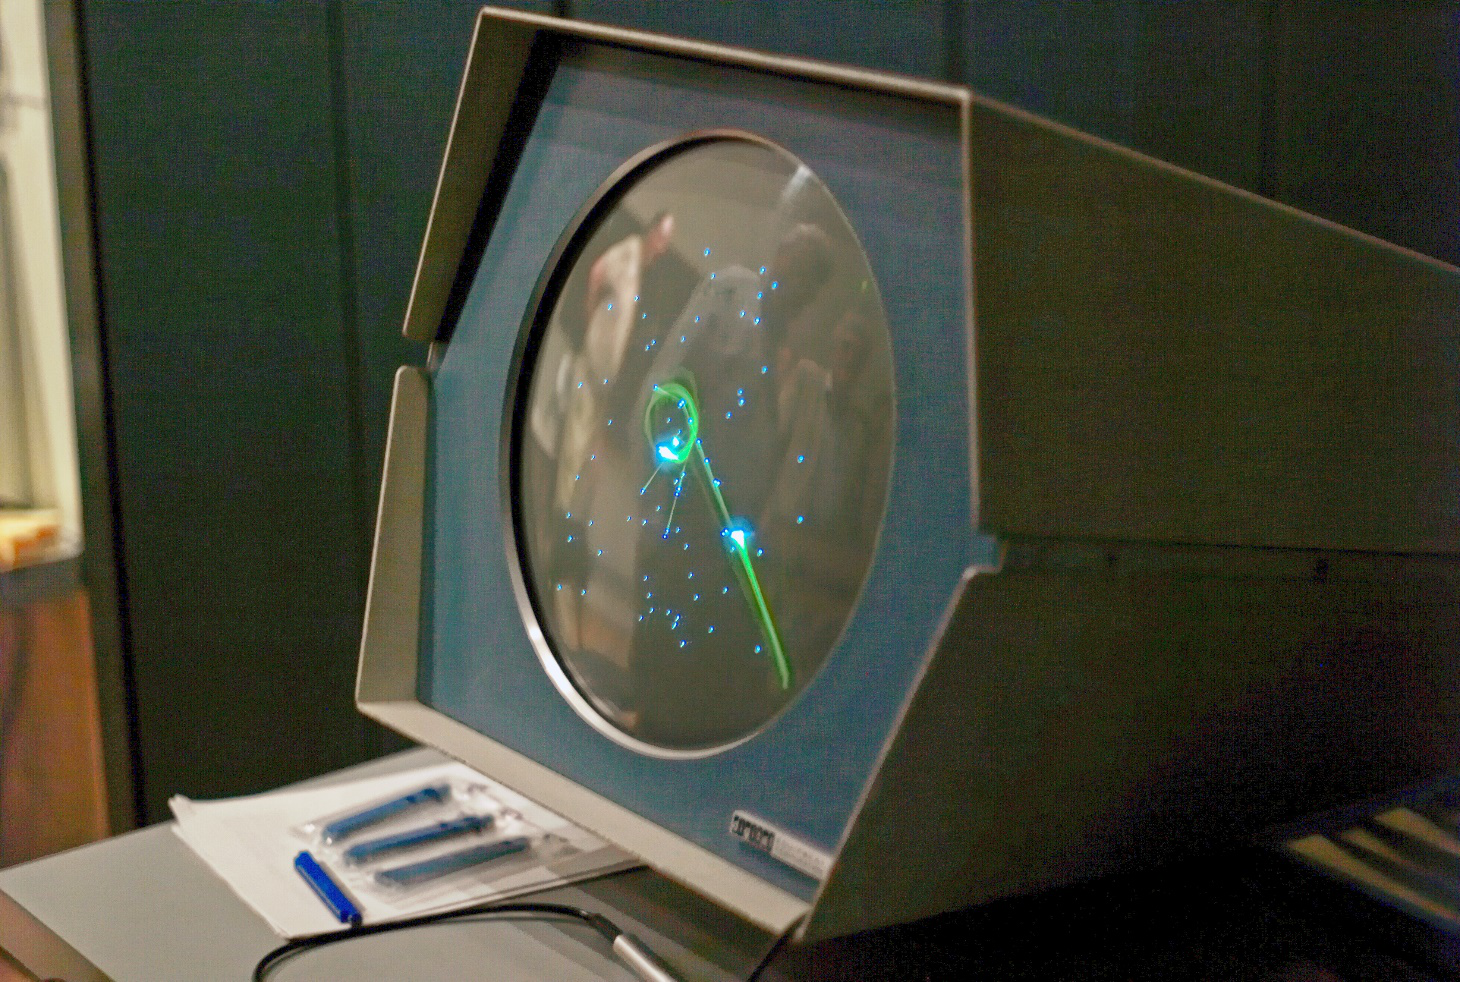
\includegraphics[width=\textwidth]{images/Spacewar.png}
			\caption {DEC PDP-1 and Spacewar}
			\end{figure}
		\end{column}
		
	\end{columns}
	
	\note{
		\textbf{ЭЛТ (Электронно-лучевая трубка)}
		
		Работает с помощью электронного пучка, испускаемого катодом (электронной пушкой) и ускоряемого анодом; на люминофорном экране пучок вызывает свечение.
		Имеет крупные размеры, высокое энергопотребление и вес, но обеспечивает хорошее качество изображения и высокую частоту обновления.
		
		% LCD (Liquid Crystal Display или жидкокристаллический дисплей)
		
		% Основан на управлении светом через жидкие кристаллы с подсветкой. Более тонкий, легкий, с меньшим энергопотреблением, но может иметь ограничения по углам обзора и контрасту.
		
		% OLED (Organic Light-Emitting Diode или органический светодиод)
		
		% Использует органические светодиоды для создания изображения. Тонкий, энергоэффективный, обеспечивает отличное качество изображения, особенно в темных сценах, но может быть подвержен эффекту выгорания пикселей (особенно на статичных изображениях).
	}
	
	\end{frame}

\begin{frame}{Кошечка (1968 г.)}{Одна из первых компьютерных анимаций}
	
	\begin{columns}
		\begin{column}{0.5\textwidth}
			
			\textbf{Авторы:} Н.\,Н. Константинов, В.\,В. Минахин, В.\,Ю. Пономаренко; оператор В. Журкин
			
			\textbf{Платформа:} БЭСМ-4 и алфавитно-цифровой принтер
			
			\textbf{Реализация:} движения кошки описаны дифференциальными уравнениями
			
		\end{column}
		\begin{column}{0.5\textwidth}
			\begin{figure}
				\href{https://www.youtube.com/watch?v=LzMk5sC6eAU}{
				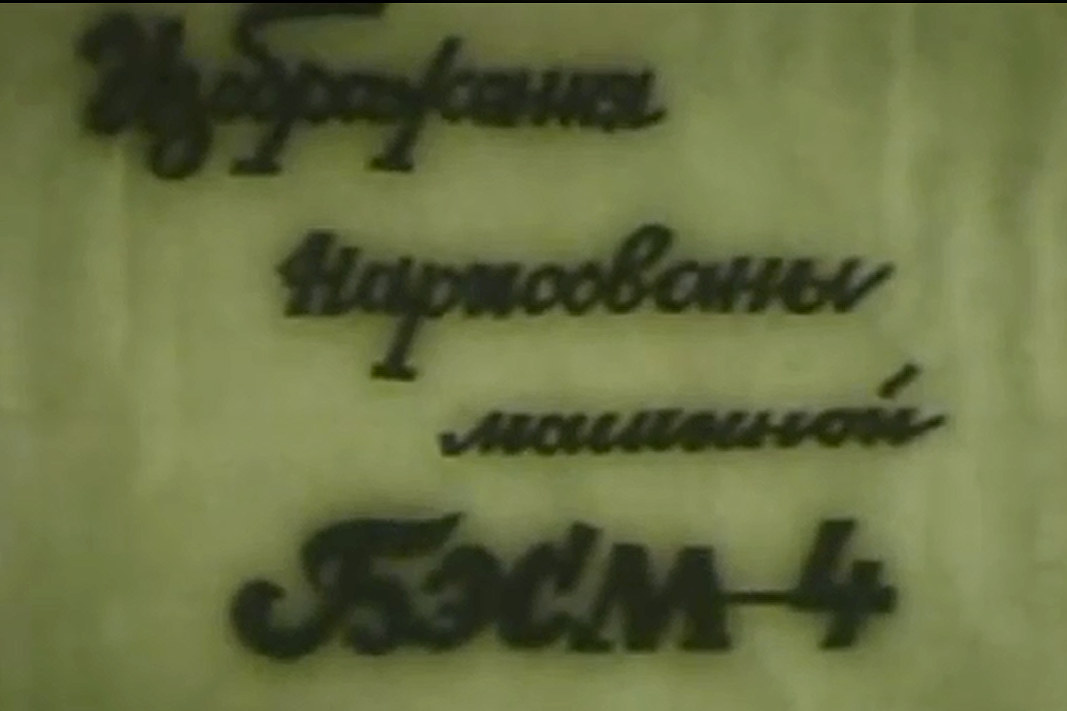
\includegraphics[width=\textwidth]{images/AnimatedCat.jpg}
				}
				\caption {Кошечка}
			\end{figure}
		\end{column}
	\end{columns}
\end{frame}

\begin{frame}{Чайник из Юты (1975 г.)}{Utah teapot, Newell teapot}
	\begin{columns}
		\begin{column}{0.5\textwidth}
			\begin{figure} 
				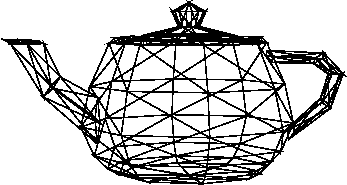
\includegraphics[width=\textwidth]{images/Utah_teapot_model.png}
				\caption {Состоит из 32 бикубических поверхностей Безье}
			\end{figure}
		\end{column}
		\begin{column}{0.5\textwidth}
			\begin{figure} 
				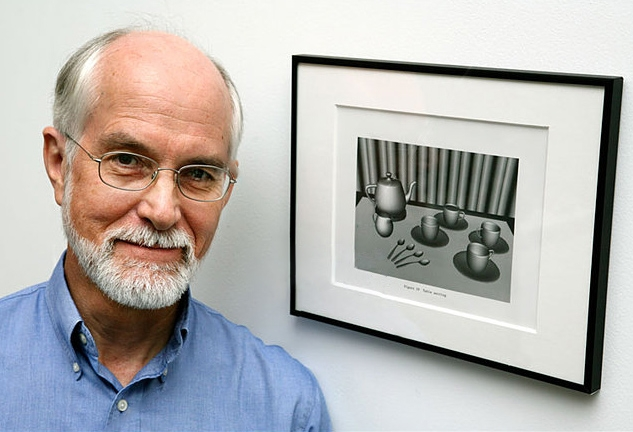
\includegraphics[width=\textwidth]{images/Utah_teapot_and_Newell.png}
				\caption {Мартин Ньюэлл и чайник из Юты}
			\end{figure}
		\end{column}
	\end{columns}

	\note{
		https://www.opengl.org/resources/libraries/glut/spec3/node89.html
		
		% Скомпилировать программу из 
		% CG/Projects/src/utah\_teapot.c
	}

\end{frame}

\begin{frame}{Silicon Graphics Inc. (SGI, 1982 г.)}{}
	\begin{columns}
		\begin{column}{0.5\textwidth}
			
			\textbf{Описание:} Разработка графических станций (Indigo, Indy и др.) и ПО (SGI IRIX и др.) для визуализации
			
			\textbf{Основатель:} Джим Кларк
			
		\end{column}
		\begin{column}{0.5\textwidth}
			\begin{figure} 
				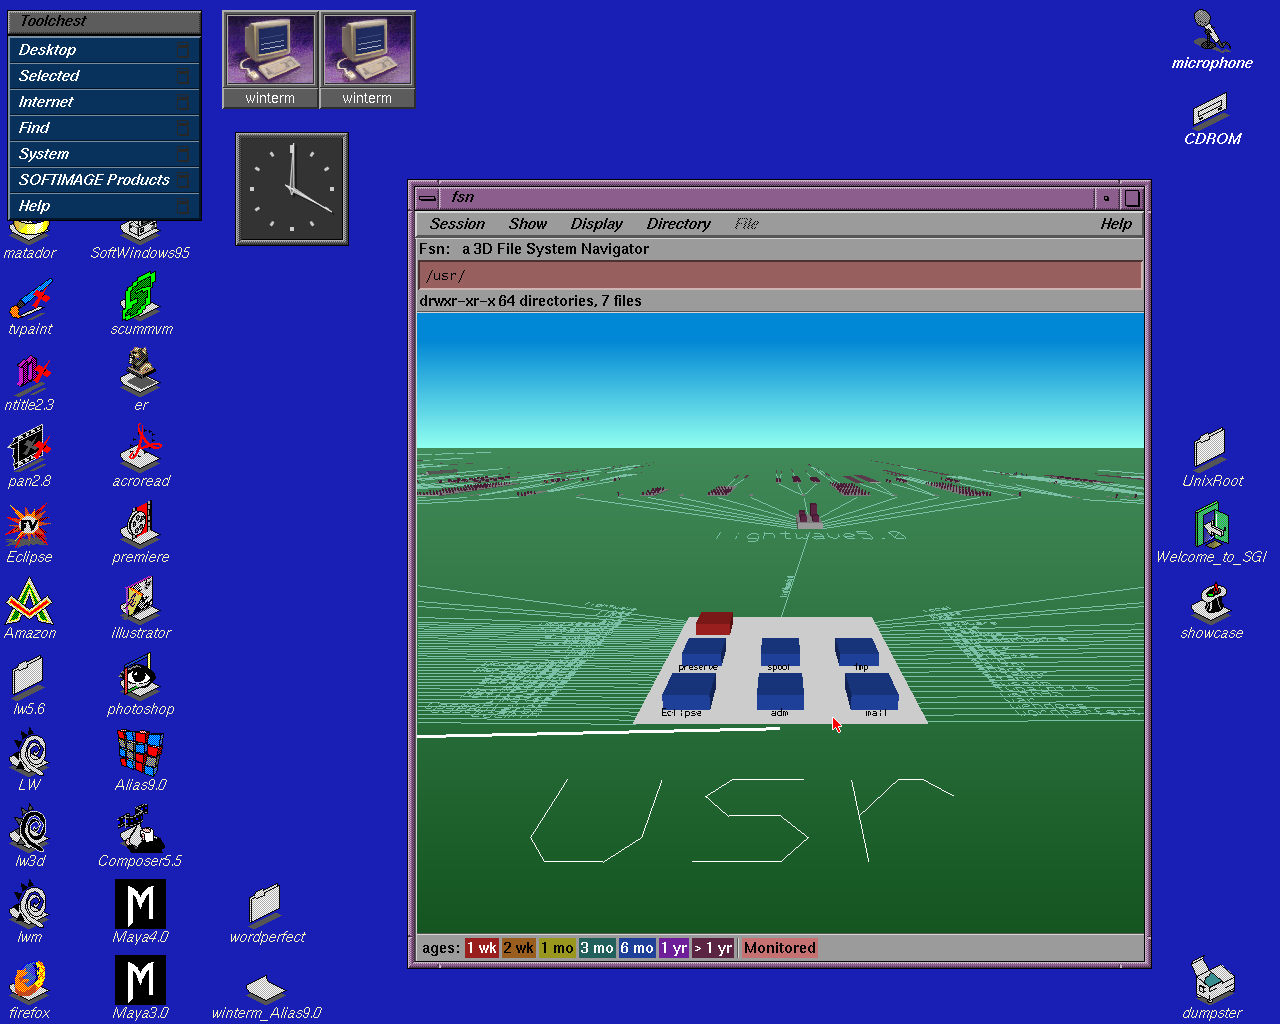
\includegraphics[width=\textwidth]{images/IRIX_OS.png}
				\caption {IRIX OS}
			\end{figure}
		\end{column}
	\end{columns}
	\note{

	
		{
		\scriptsize

		\textbf{История компании Silicon Graphics}

		https://habr.com/ru/companies/vdsina/articles/562912/	

		В 1984 году SGI выпустила системы IRIS первого поколения (модели 1000 и 1200).

		Вскоре получила статус легенды среди 3D-художников и графических дизайнеров, использовавших уникальную мощь её рабочих станций.

		Наследие SGI можно увидеть в Nintendo 64 (вышла в 1996 г.). 
		
		Рабочие станции SGI использовались при создании голливудских фильмов, включая 
		Jurassic Park, «Парк юрского периода» (1993 г.),
		Jumanji, «Джуманджи» (1995 г.),
		The Matrix, «Матрица» (1999 г.),
		Star Wars. Episode I, «Звёздные войны. Эпизод I» (1999 г.),
		Lord of the Rings, «Властелин колец» (2001 г.),
		и другие.

		В 1992 году SGI решила перепроектировать API и начала продавать недорогие лицензии на него своим конкурентам.
		После этого SGI организовала OpenGL Architecture Review Board для руководства дальнейшими разработками.

		В феврале 1996 года SGI решила войти на рынок суперкомпьютеров, приобретя за 740 миллионов долларов Cray Research.

		В 2003 году компания освободила помещения своей штаб-квартиры в Маунтин-Вью и сдала здание в аренду Google.

		В апреле 2009 года SGI снова подала заявление о банкротстве по главе 11 и была продана Rackable Systems за 25 миллионов.
		
		\_
		
		}
	}

\end{frame}


\begin{frame}{Массовый 3D-ускоритель (1996 г.)}{3dfx Voodoo Graphics}
	\begin{columns}
		\begin{column}{0.5\textwidth}
			
			\begin{figure}
				\href{https://www.youtube.com/watch?app=desktop&v=Zdf270cZD9g}{
				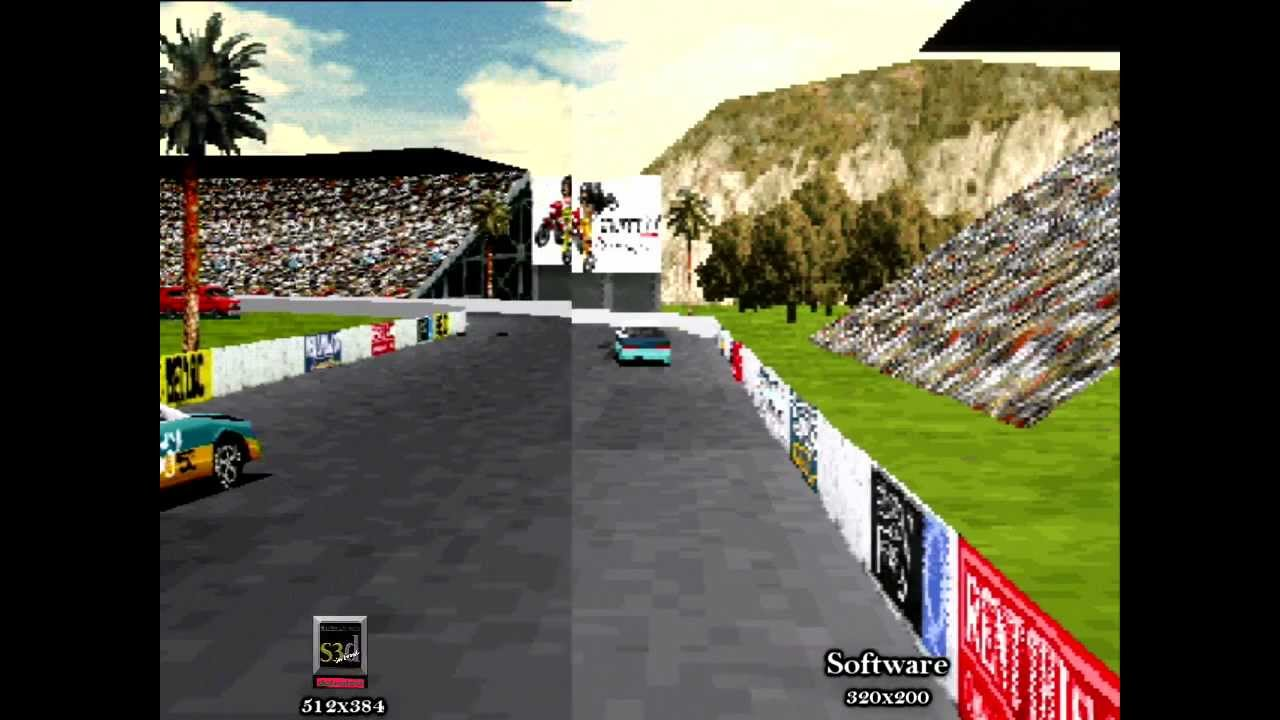
\includegraphics[width=\textwidth]{images/Destruction_Derby_1995.png}}
				\caption {Destruction Derby (1995 г.)}
			\end{figure}
		\end{column}
		\begin{column}{0.5\textwidth}
			\begin{figure} 
				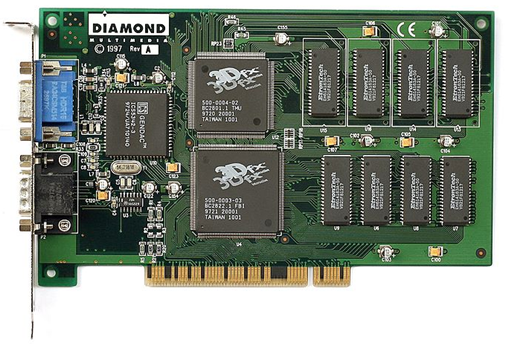
\includegraphics[width=\textwidth]{images/Diamond_Monster_3D_3DFX_Voodoo1.png}
				\caption {Diamond Monster 3DFX Voodoo1}
			\end{figure}
		\end{column}
	\end{columns}

	\note{
		\textbf{Характеристики видеокарты}
		\vspace{0.5em}

		\textbf{Разработчик чипсета:} 3Dfx Interactive

		\textbf{Производитель платы:} Diamond Multimedia
			
		\textbf{Шина:} PCI (VGA pass-through)
		
		\textbf{Память:} 4 MB EDO DRAM
		
		\textbf{Техпроцесс:} 500 nm
		
		\textbf{Частота min/max:} 45/50 MHz
		
		\textbf{API:} Glide (позднее Direct3D)
		
		\textbf{Цена:} 300\$
		
		\textbf{Эффекты:} texture modulation, Z-buffering, bi-linear texture filtering, anti-aliasing и др.
	}
\end{frame}

\end{document}
